\section{Numerical Implementation}
\label{sec:numerical_imp}

First, I test the proposed PINN tomography framework on synthetic examples and then compare the results with the traditional gradient-based traveltime tomography. All PINN enabled tomography implementations are conducted in TensorFlow. For the training, ADAM optimizer~\cite{kb:14} with a default learning rate of 0.001 is chosen before switching to the L-BFGS ~\cite{ln:89} method for the sake of accelerating the convergence. In order to save computational time, all training is performed with a minibatch implementation in which the collocation points are randomly selected from the computational domain using a Latin hypercube sampling ~\cite{s:87}.

The first model example representing a near-surface is a three-layered model with minor folds (\figref{fig:folded_model}). The model size is assumed 36 $\times$ 211 and sampled with a uniform spacing of 10 m both vertically and horizontally ($\Delta z = \Delta x = 10 \, m$). To model the traveltimes, I employ the fast marching method. I use 43 shots with a regular interval of 50 m on the surface.  There are 211 receivers for each shot which makes 43$\times$211 observed surface traveltime data for the PINN implementation (\figref{fig:folded_data}).

 
\begin{figure}
       \centering
       \begin{subfigure}[b]{.9\textwidth}
               \centering
               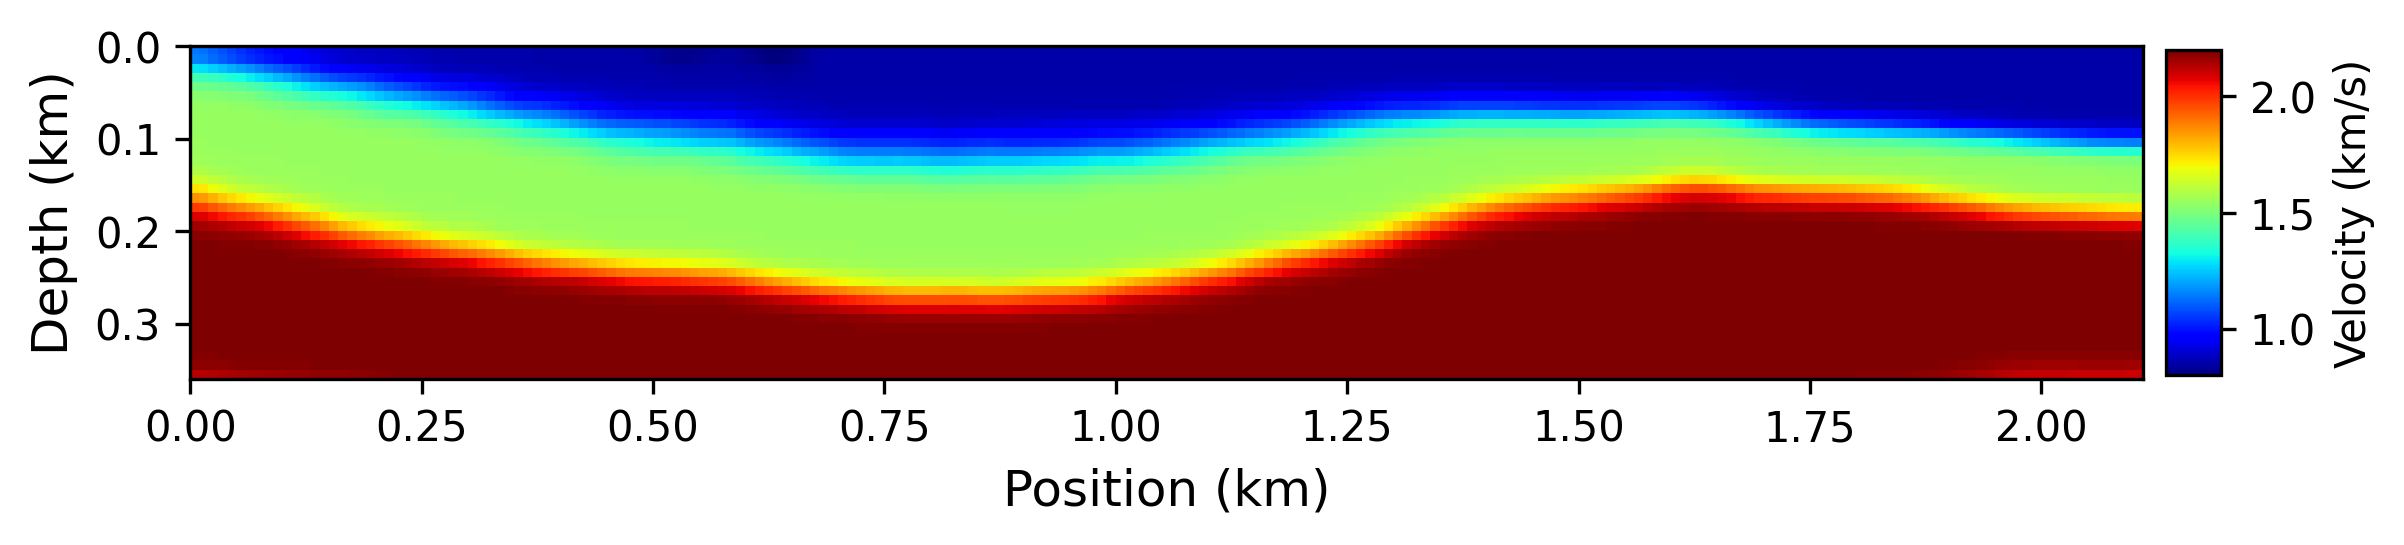
\includegraphics[width=0.9\textwidth]{figures/chap03_pinn_enabled/folded_model} 
               \caption{}
               \label{fig:folded_model}
       \end{subfigure}
       \begin{subfigure}[b]{.9\textwidth}
               \centering
               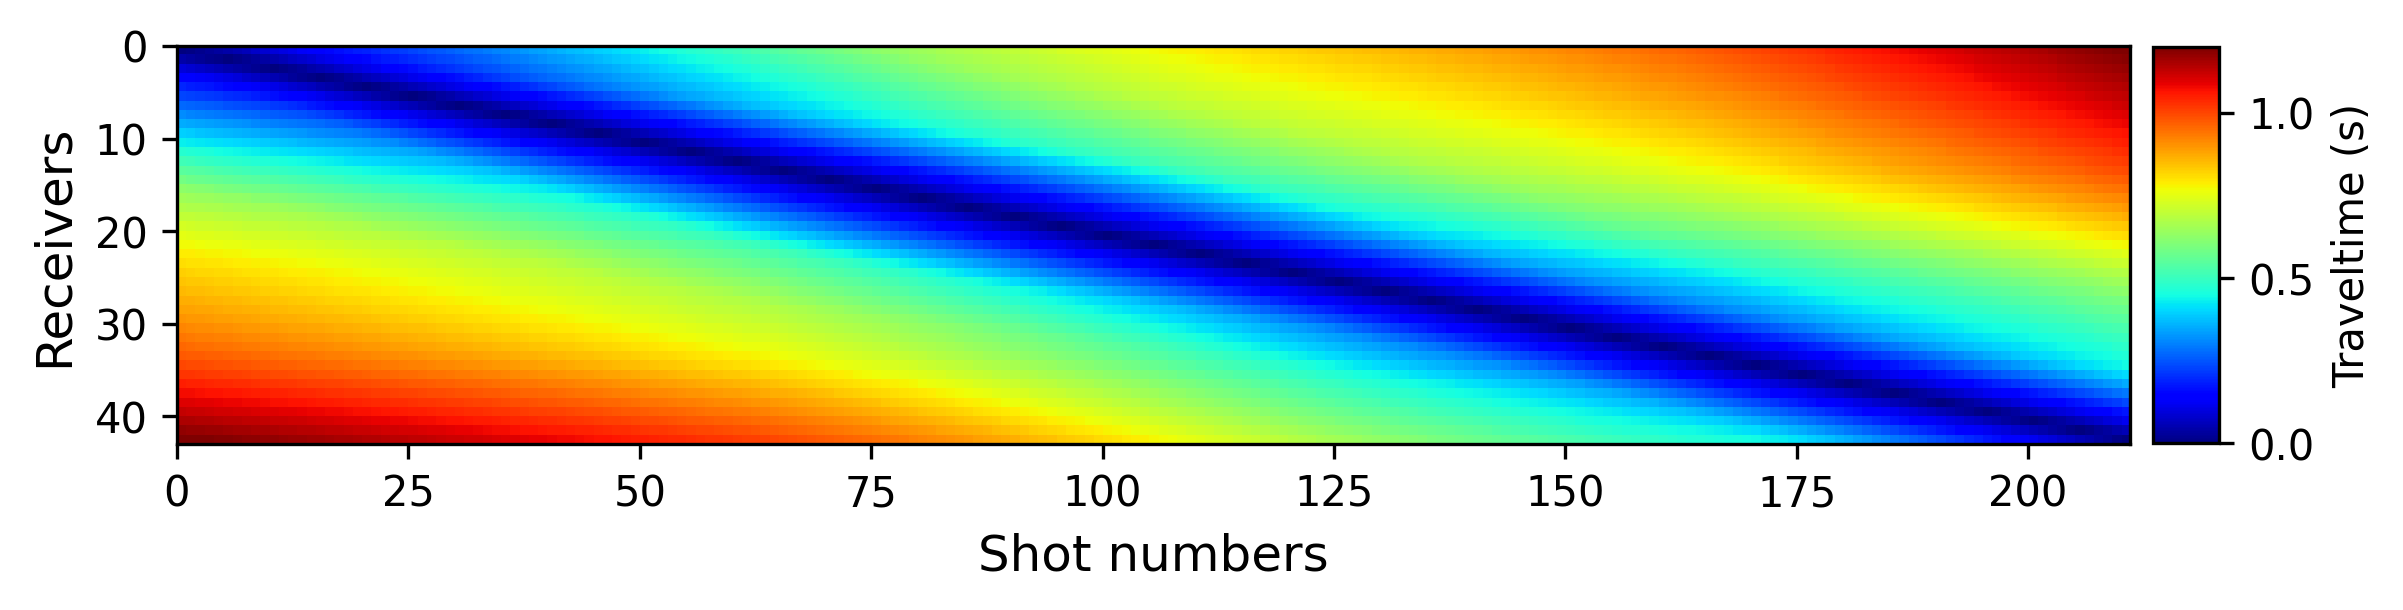
\includegraphics[width=0.9\textwidth]{figures/chap03_pinn_enabled/folded_data}
               \caption{}
               \label{fig:folded_data}
       \end{subfigure}
       \caption{(a) An example of a velocity model for testing the proposed PINN enabled inversion and (b) Image representation of the data aquired from the model. There are 43 shots each having 211 observed traveltimes that are placed in rows to form the image.  }
       \label{fig:folded_example}
\end{figure}


I choose 300 samples from the computational domain with the Latin hypercube sampling method to train the model. After examining the outputs of different settings of the hyperparameters, I use the following tunings: 7 hidden layers with 50 neurons each are used for the traveltime network, while for the velocity, 5 hidden layers with 50 neurons each are decided sufficient as training the velocity network is easier than training the traveltime network. The weight for the TV term is chosen as $\lambda = 10^{-7}$. Moreover, I use $\alpha = 100$ as the weight for the data mismatch term in the loss. Penalizing this specific term during the training helps to improve the accuracy of the retrieved model. The neural network weights are initialized with Xavier initializer~\cite{gb:10}. The estimated velocity model after 20,000 ADAM iterations (\figref{fig:folded_loss_curve}) which is followed by the L-BFGS is shown in \figref{fig:pinn_folded_result}. The retrieved model successfully captures the main features of the true model (\figref{fig:folded_model}). To give a comparison, I additionally perform traditional traveltime tomography using the conjugate-direction (CD) method ~\cite{c:14}. The acquisition geometry is the same as for the PINN tomography and the tomographic inversion is obtained by implementing 10 linearization updates each having 30 conjugate-gradient iterations. The convergence history for the traditional approach is presented in \figref{fig:convergence_curve1}. Starting velocity model for the inversion is obtained by taking the vertical profile from the true model (\figref{fig:folded_model}) and then applying strong smoothing. The inverted model and the initial one is given in \figref{fig:std_tomo1}. Even though the inversion is started with a priori knowledge of the vertical profile from the region, the inversion can not approach the true velocities in many places as the optimization traps in local minimum points.

\begin{figure}
 \centering
 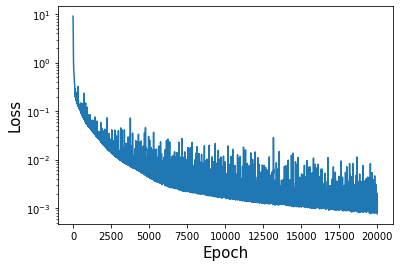
\includegraphics[width=0.7\textwidth]{figures/chap03_pinn_enabled/folded_loss_curve} 
 \caption{Loss curve of the PINN tomography after 20,000 ADAM iterations using minibatch implementation with a batch size of 300.}
 \label{fig:folded_loss_curve}
\end{figure}


\begin{figure}
 \centering
 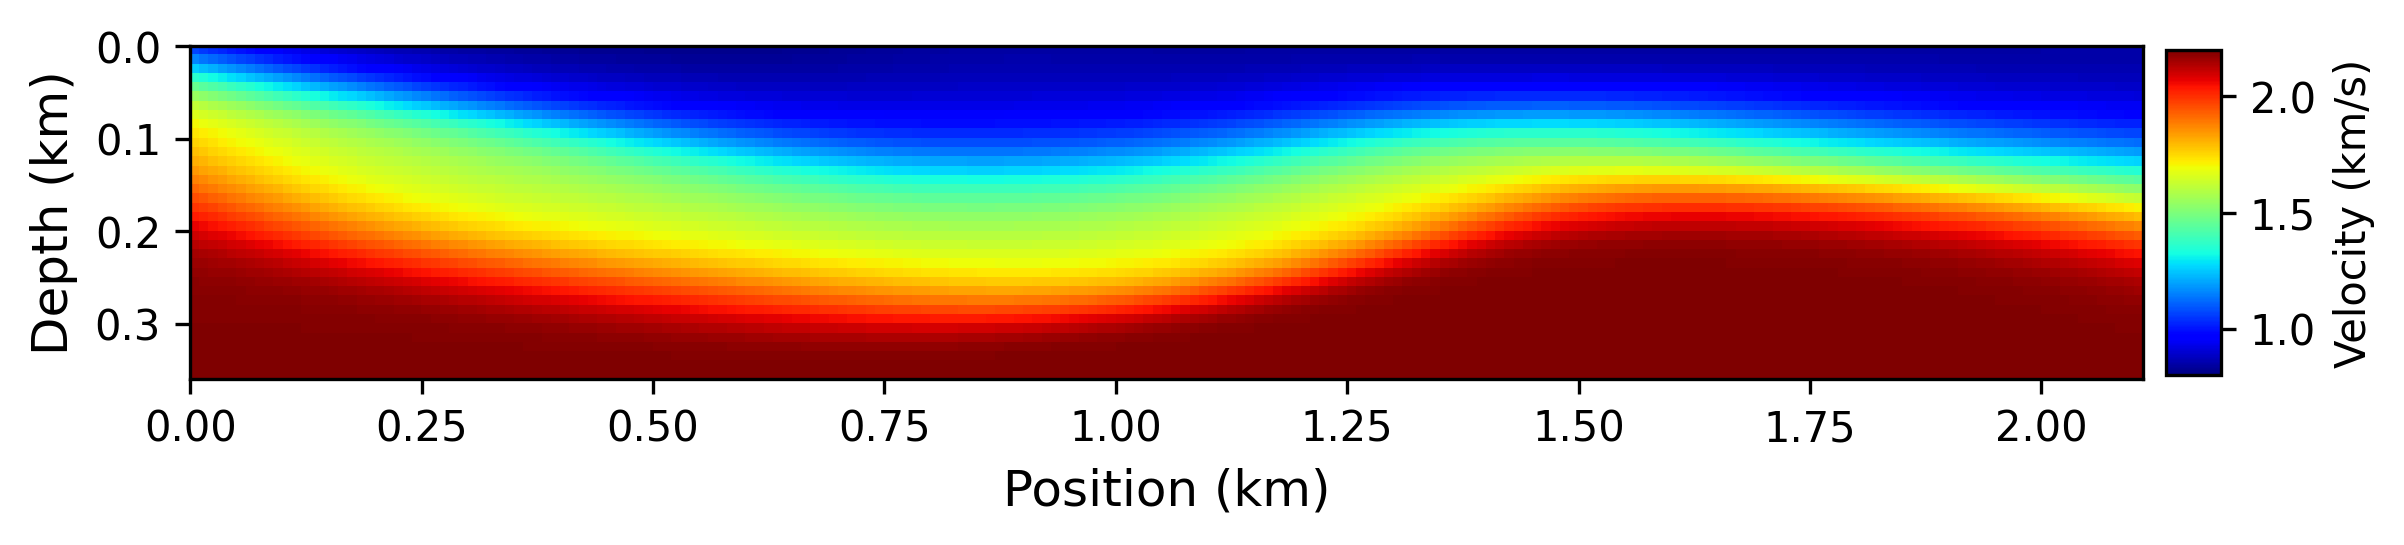
\includegraphics[width=1.0\textwidth]{figures/chap03_pinn_enabled/pinn_folded_result} 
 \caption{PINN predicted velocity model after L-BFGS iterations.}
 \label{fig:pinn_folded_result}
\end{figure}

\begin{figure}
 \centering
 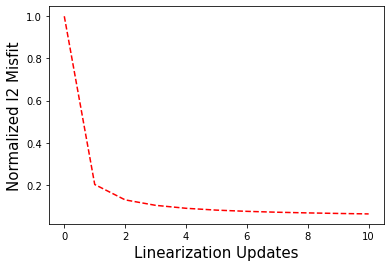
\includegraphics[width=0.7\textwidth]{figures/chap03_pinn_enabled/convergence_curve1} 
 \caption{Convergence history of the gradient-based tomography after 10 linearization updates. 30 conjugate-gradient iterations are used for each linearization.}
 \label{fig:convergence_curve1}
\end{figure}

\begin{figure}
       \centering
       \begin{subfigure}[b]{1.\textwidth}
               \centering
               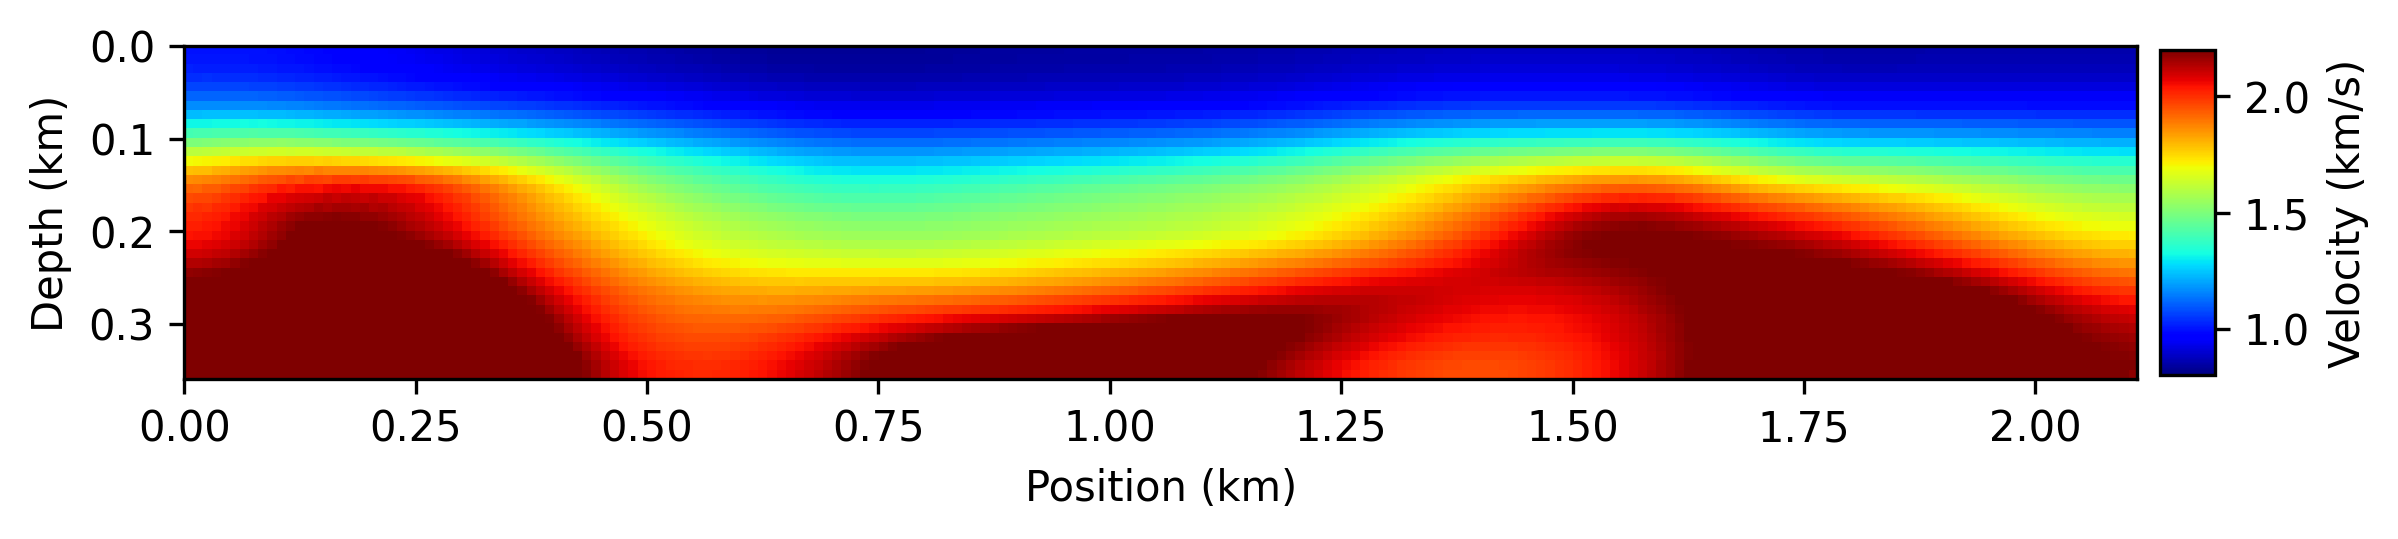
\includegraphics[width=0.9\textwidth]{figures/chap03_pinn_enabled/folded_tomo} 
               \caption{}
               \label{fig:folded_tomo}
       \end{subfigure}
       \begin{subfigure}[b]{1.\textwidth}
               \centering
               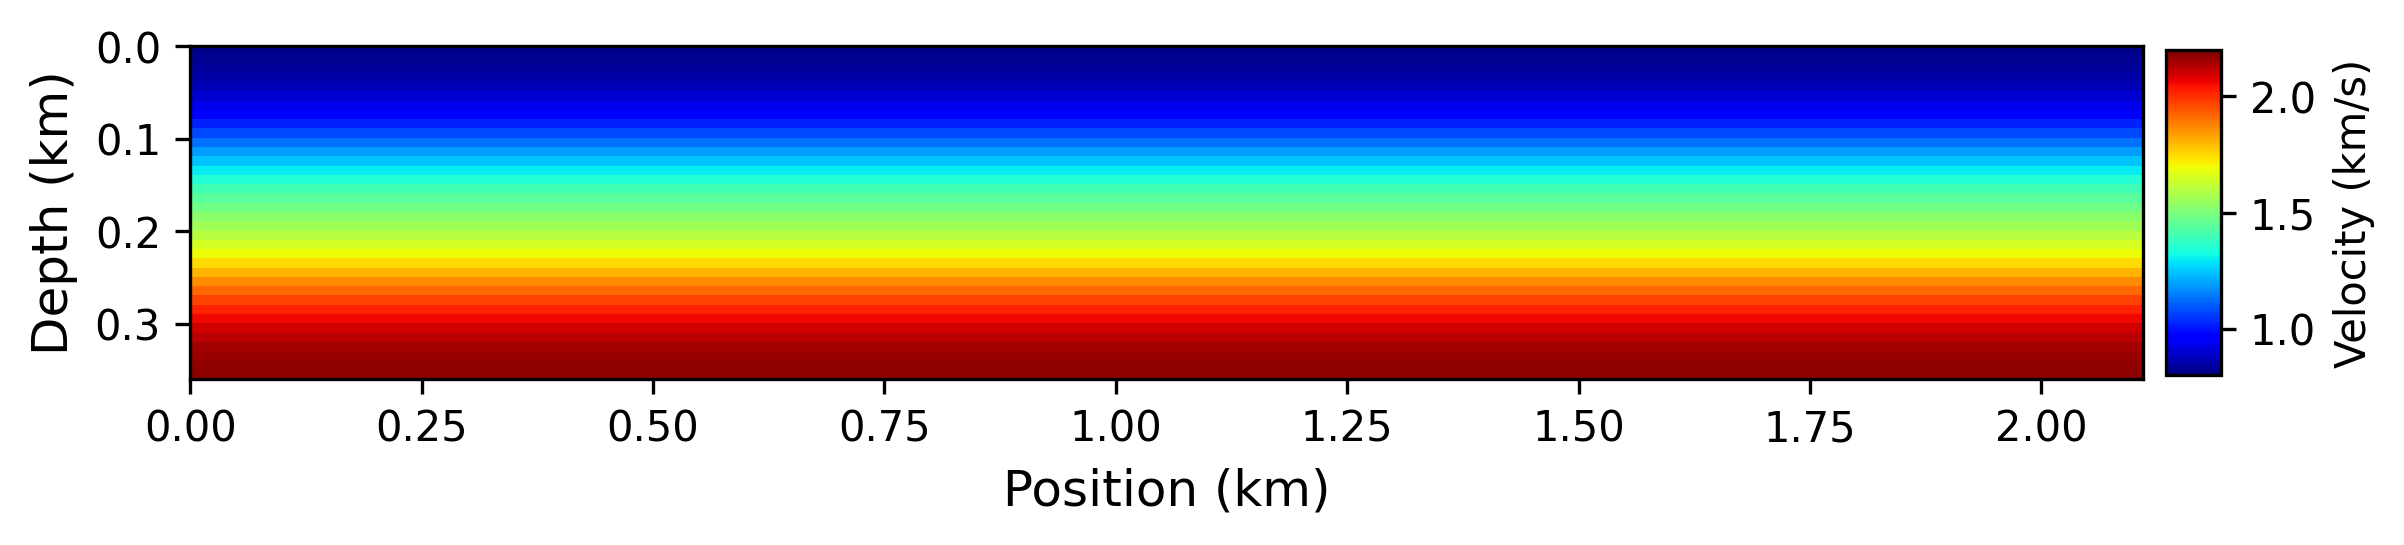
\includegraphics[width=0.9\textwidth]{figures/chap03_pinn_enabled/folded_init}
               \caption{}
               \label{fig:folded_init}
       \end{subfigure}
       \caption{(a) Inverted model from the conventional tomography and (b) Starting velocity model for tomography.}
       \label{fig:std_tomo1}
\end{figure}

The next example for testing the proposed approach is a more complicated near-surface model containing fault systems (\figref{fig:thesis_model2}). The acquisition parameters selected in the first example is again employed for acquiring the data (\figref{fig:thesis_model2_data}). This time, PINN inversion is performed by using 40,000 Adam iterations  (\figref{fig:thesis_model2_loss}) with a minibatch size of 500 and followed by the L-BFGS algorithm. The final inversion result is provided in \figref{fig:thesis_model2_pinn}. Again for comparison, traditional tomography is implemented. No further improvement in the convergence is observed after the 10th linearization step (\figref{fig:convergence_curve2}). Although the inverted model (\figref{fig:model2_tomo}) is generally similar to the predicted model by the PINN  (\figref{fig:thesis_model2_pinn}), it presents wrongly estimated high velocities some of the areas in the model maybe bacause of the contradicting gradient information along the shot dimension. To present a quantitative assessment of the results from both examples, I compare vertical velocity profiles obtained from four different positions (\figref{fig:example_1_profiles}) (\figref{fig:example_2_profiles}) as well as the percent error maps (\figref{fig:error}). As expected from the traveltime tomography, both methods provide a smooth representation of the actual models. However, in deeper parts of the models traditional approach tends to deviate from the true velocities, which is especially observable for the first example. As expected from the traveltime tomography, both methods provide a smooth representation of the actual models. However, in deeper parts of the models traditional approach tends to deviate from the true velocities, which is especially observable for the first example. Also, the percentage velocity errors from the PINN-based approach are generally lower than the errors from the classical method.
\begin{figure}
       \centering
       \begin{subfigure}[b]{.9\textwidth}
               \centering
               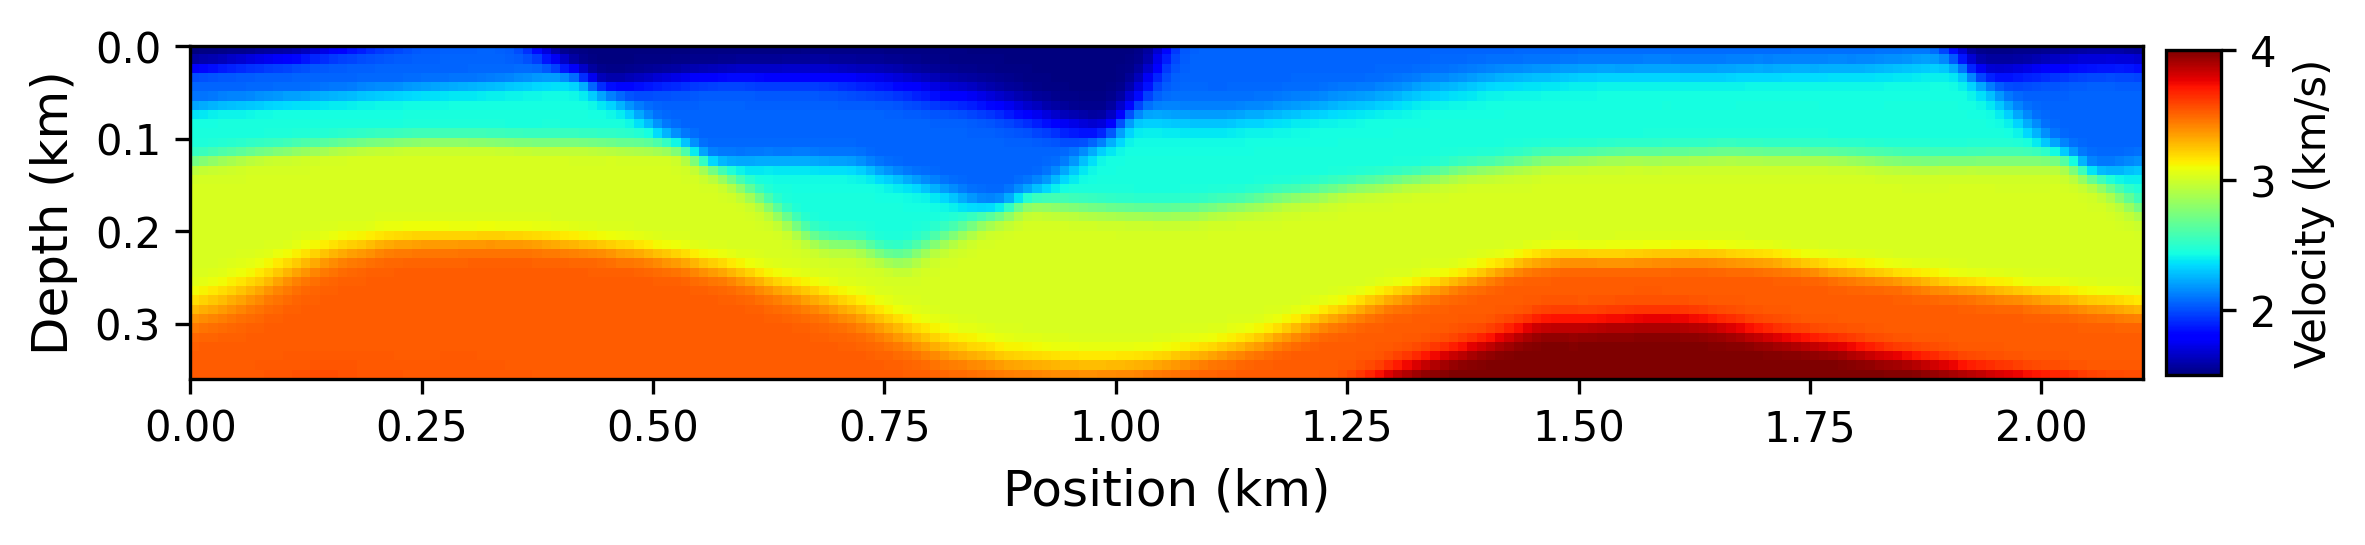
\includegraphics[width=0.9\textwidth]{figures/chap03_pinn_enabled/thesis_model2} 
               \caption{}
               \label{fig:thesis_model2}
       \end{subfigure}
       \begin{subfigure}[b]{.9\textwidth}
               \centering
               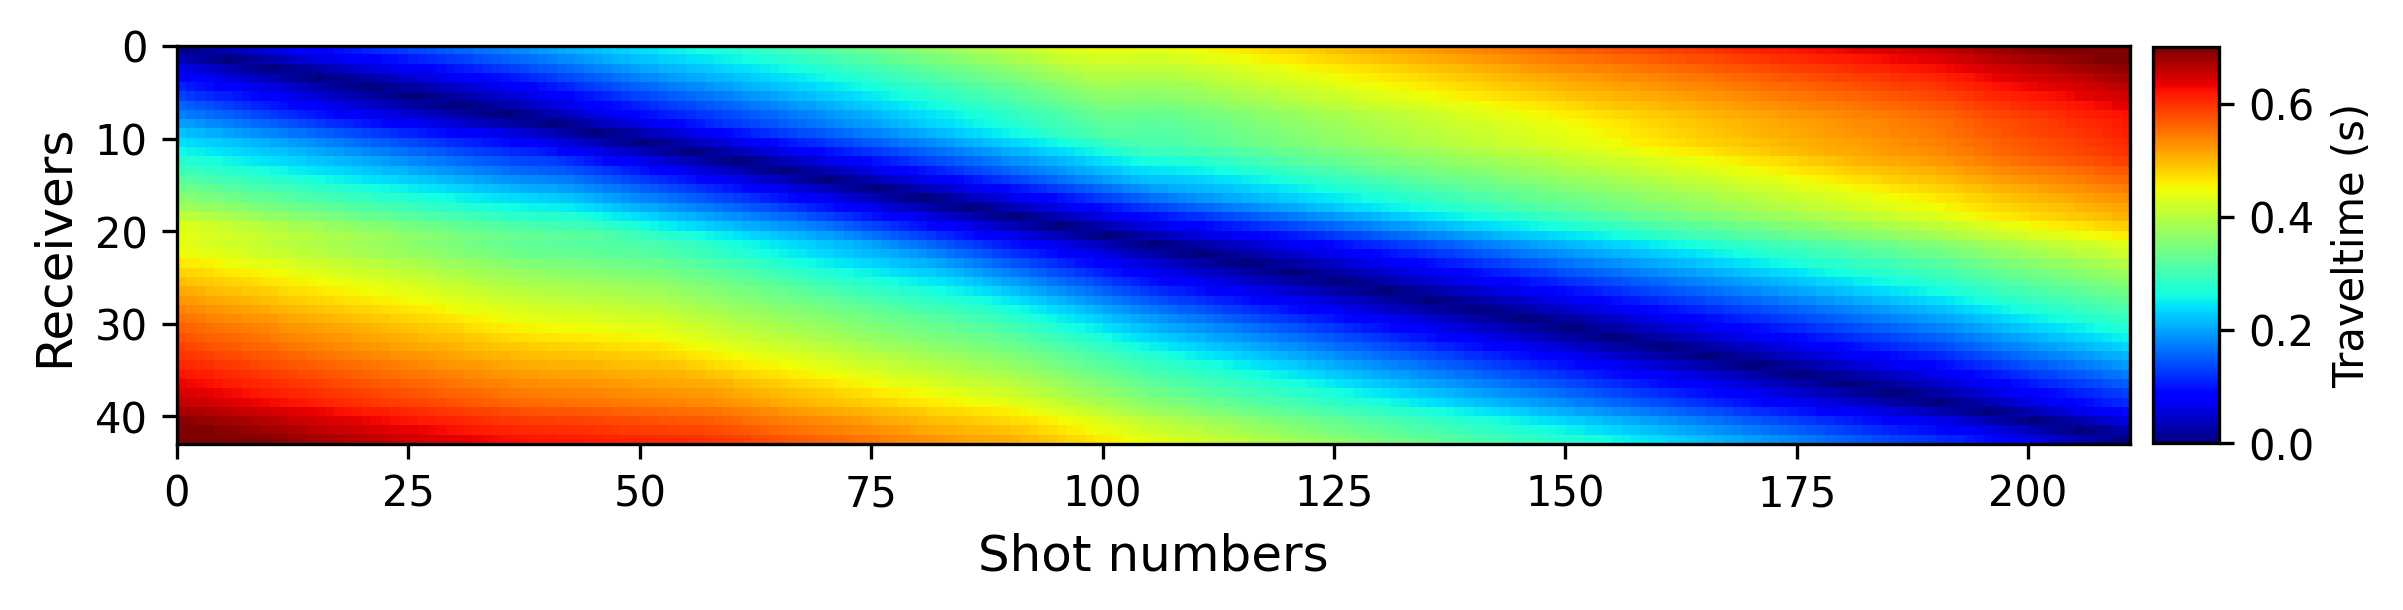
\includegraphics[width=0.9\textwidth]{figures/chap03_pinn_enabled/thesis_model2_data}
               \caption{}
               \label{fig:thesis_model2_data}
       \end{subfigure}
       \caption{(a) An example of a velocity model for testing the proposed PINN enabled inversion and (b) Image representation of the data aquired from the model. There are 43 shots each having 211 observed traveltimes that are placed in rows to form the image.  }
       \label{fig:model2}
\end{figure}

\begin{figure}
 \centering
 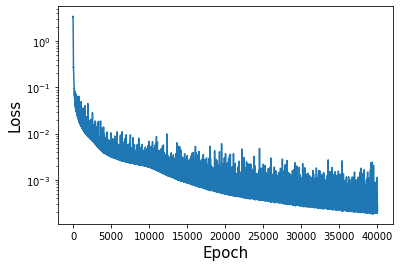
\includegraphics[width=0.7\textwidth]{figures/chap03_pinn_enabled/thesis_model2_loss} 
 \caption{Loss curve of the PINN tomography after 40,000 ADAM iterations using minibatch implementation with a batch size of 500.}
 \label{fig:thesis_model2_loss}
\end{figure}

\begin{figure}
 \centering
 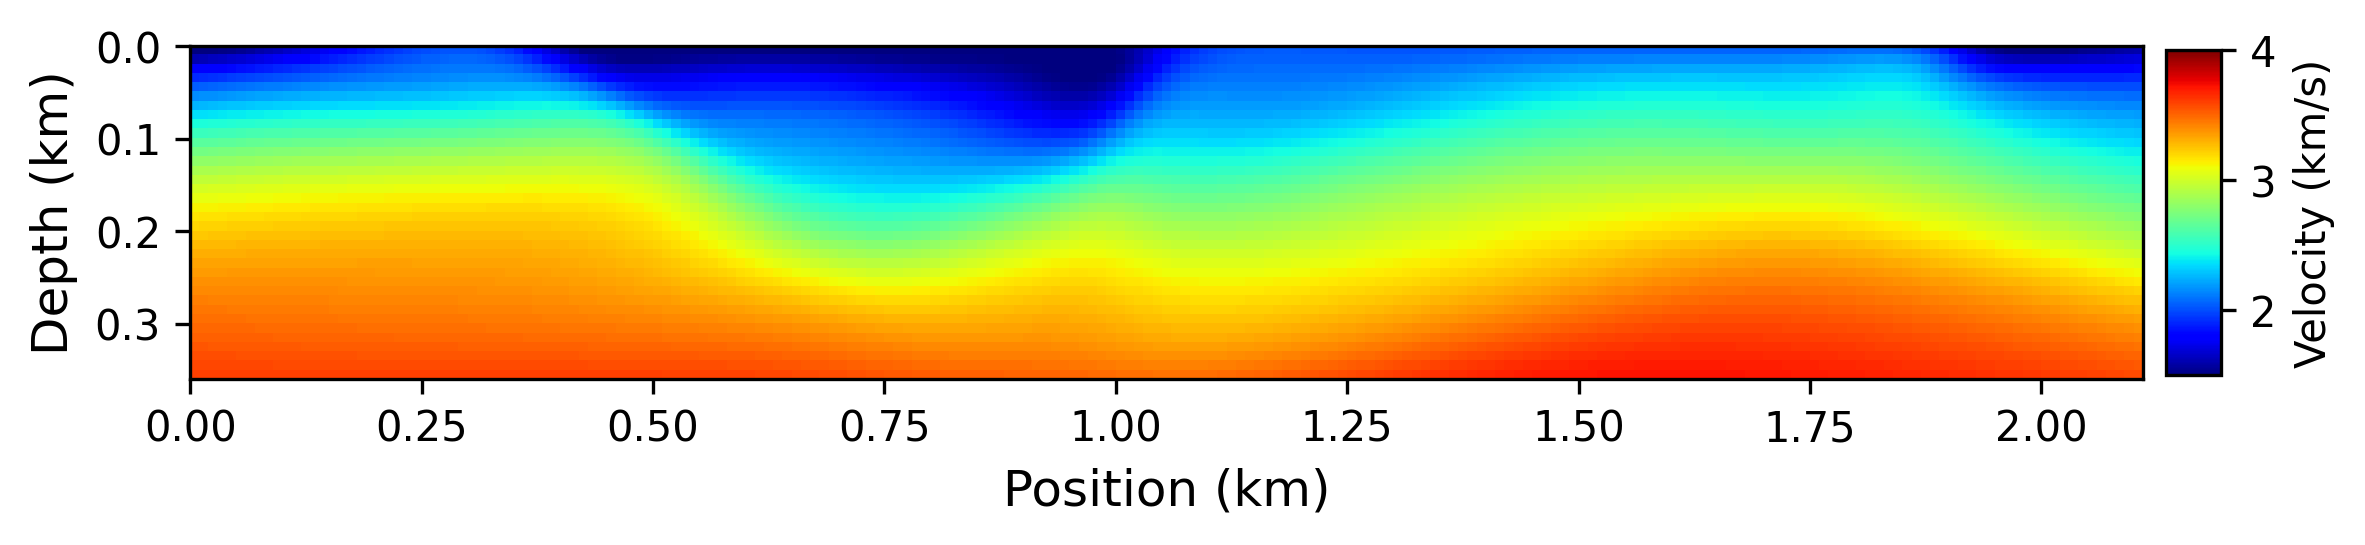
\includegraphics[width=1.0\textwidth]{figures/chap03_pinn_enabled/thesis_model2_pinn} 
 \caption{PINN predicted velocity model after L-BFGS iterations.}
 \label{fig:thesis_model2_pinn}
\end{figure}

\begin{figure}
 \centering
 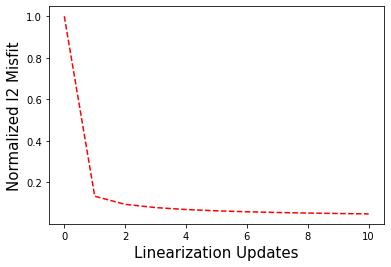
\includegraphics[width=0.7\textwidth]{figures/chap03_pinn_enabled/convergence_curve2} 
 \caption{Convergence history of the gradient-based tomography after 10 linearization updates. 30 conjugate-gradient iterations are used for each linearization.}
 \label{fig:convergence_curve2}
\end{figure}

\begin{figure}
       \centering
       \begin{subfigure}[b]{1.\textwidth}
               \centering
               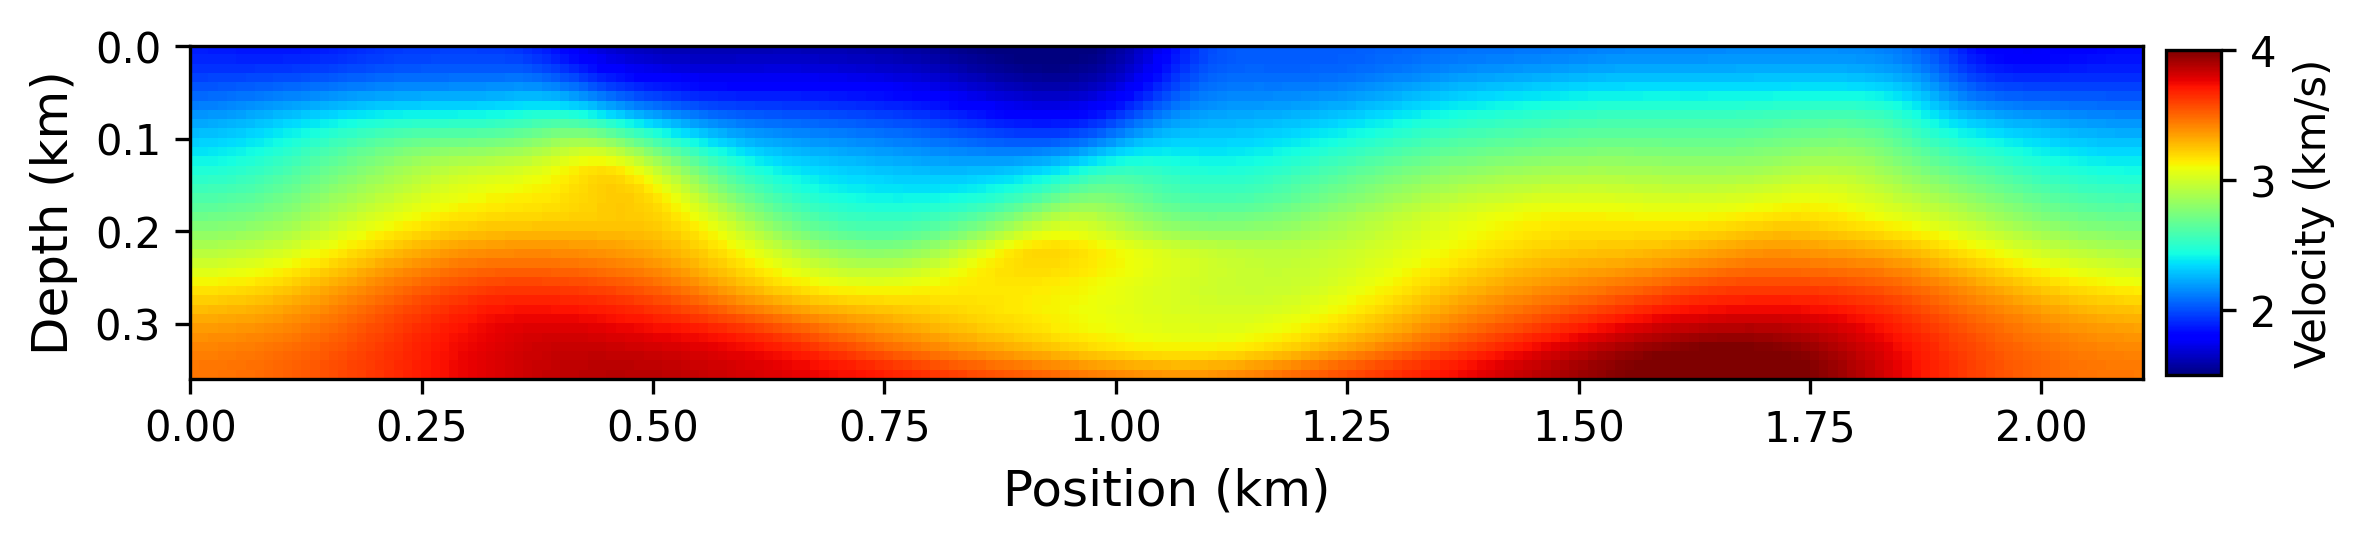
\includegraphics[width=0.9\textwidth]{figures/chap03_pinn_enabled/model2_tomo} 
               \caption{}
               \label{fig:model2_tomo}
       \end{subfigure}
       \begin{subfigure}[b]{1.\textwidth}
               \centering
               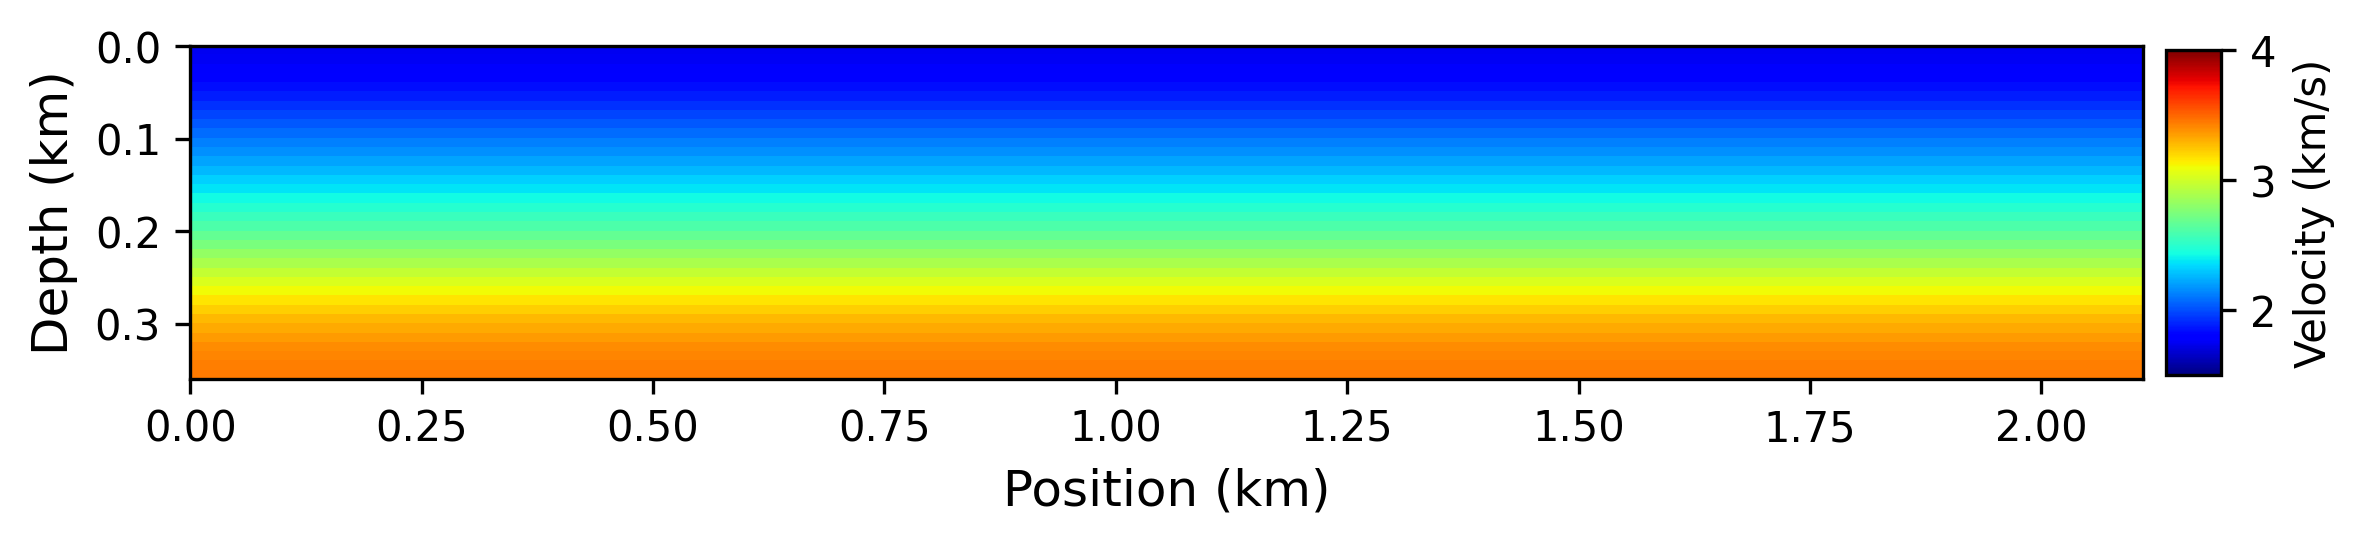
\includegraphics[width=0.9\textwidth]{figures/chap03_pinn_enabled/model2_init}
               \caption{}
               \label{fig:model2_init}
       \end{subfigure}
       \caption{(a) Inverted model from the conventional tomography and (b) Starting velocity model for tomography.}
       \label{fig:std_tomo2}
\end{figure}

\begin{figure}
 \centering
 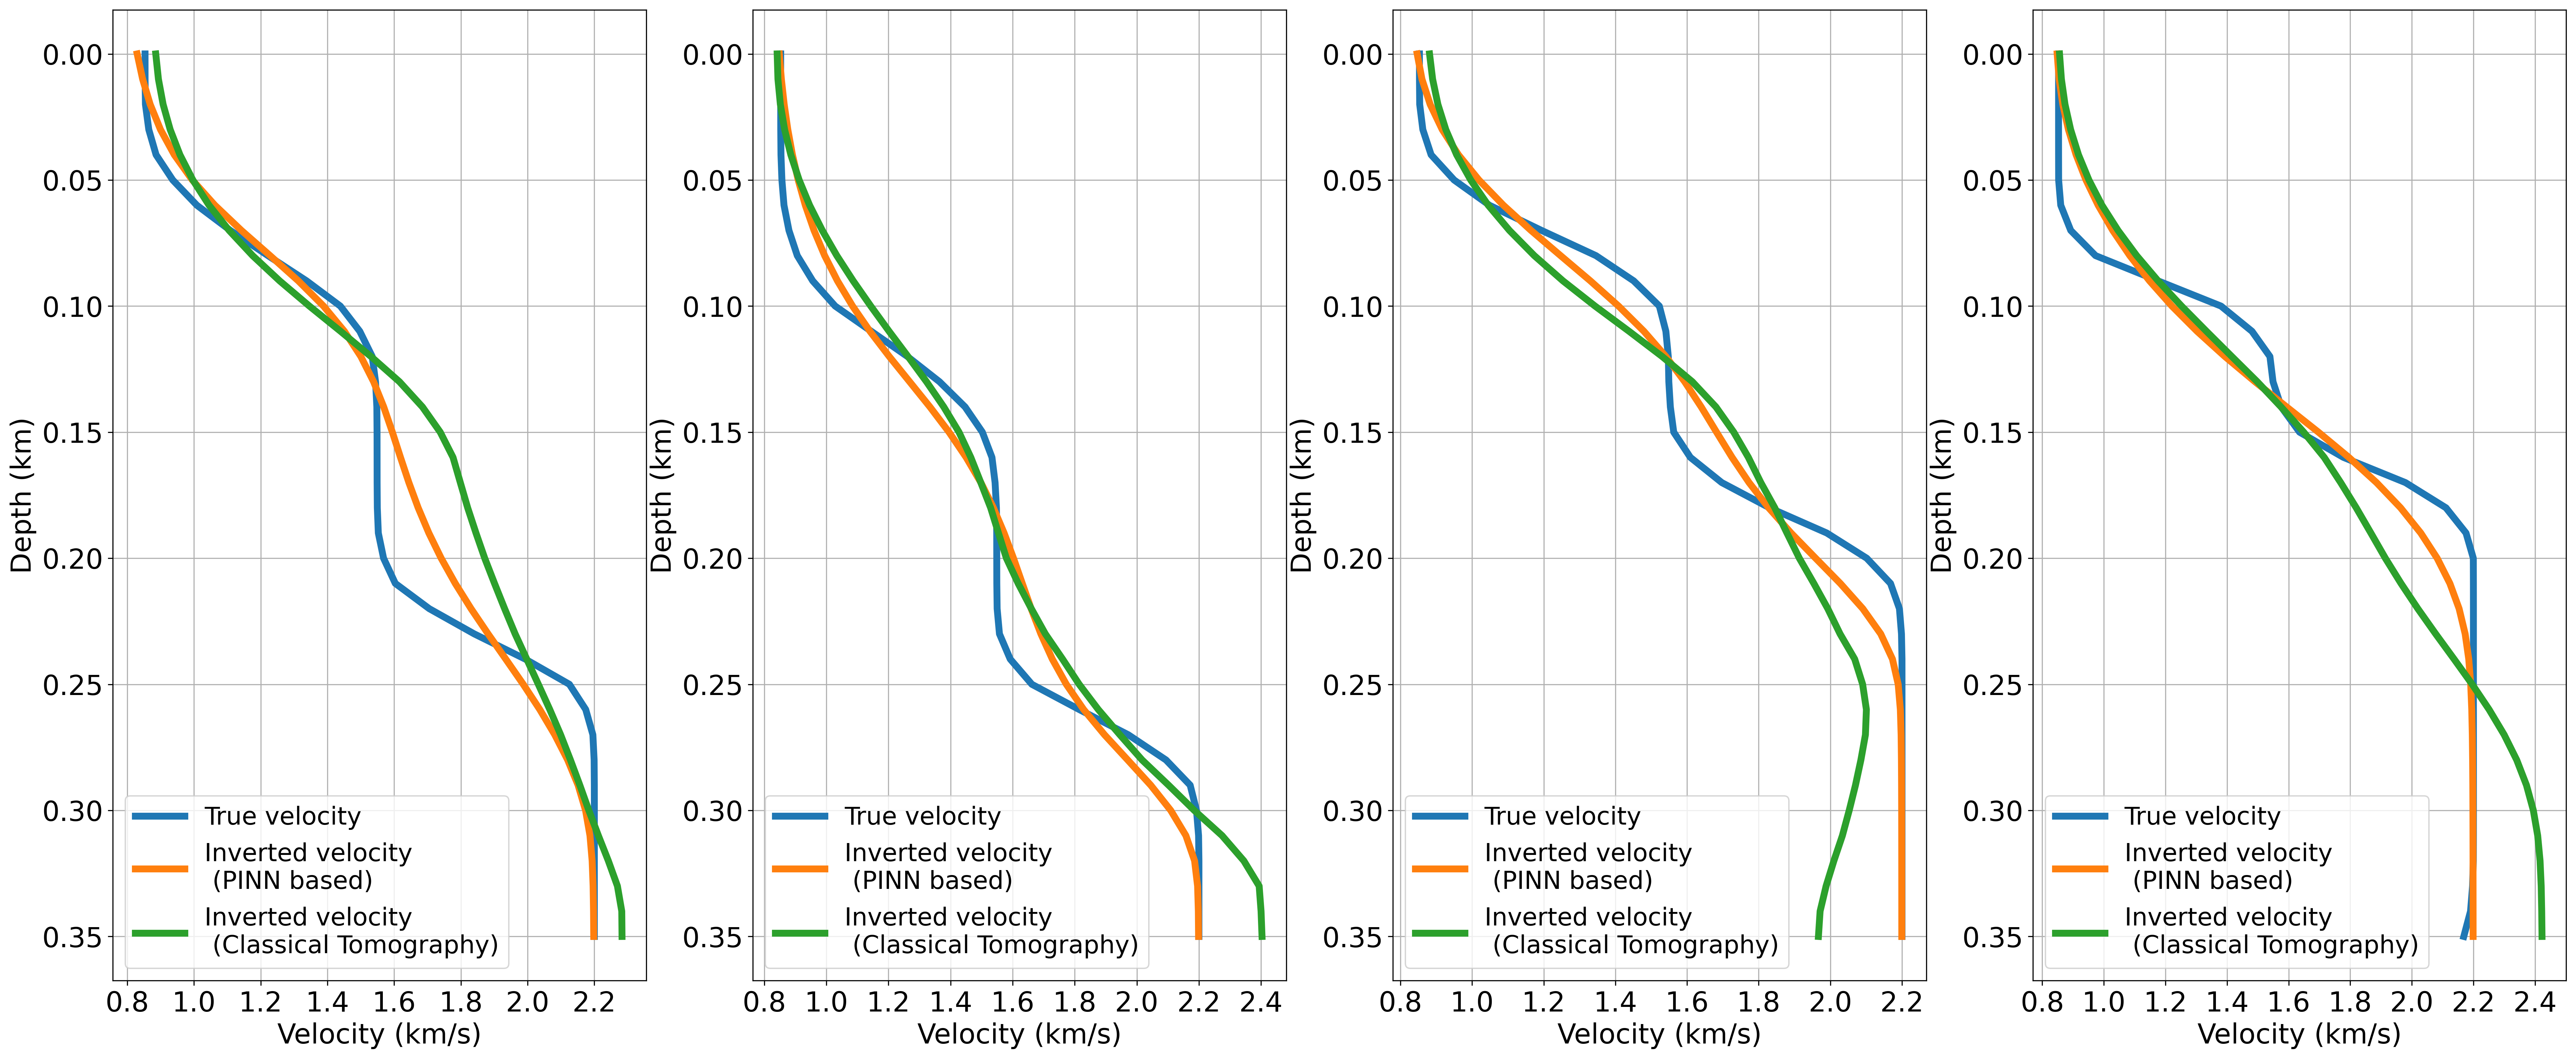
\includegraphics[width=0.9\textwidth]{figures/chap03_pinn_enabled/example_1_profiles} 
 \caption{Vertical velocity profiles at 0.4 km, 0.9 km, 1.3 km and 1.9 km from left to right respectively for the first example.}
 \label{fig:example_1_profiles}
\end{figure}

\begin{figure}
 \centering
 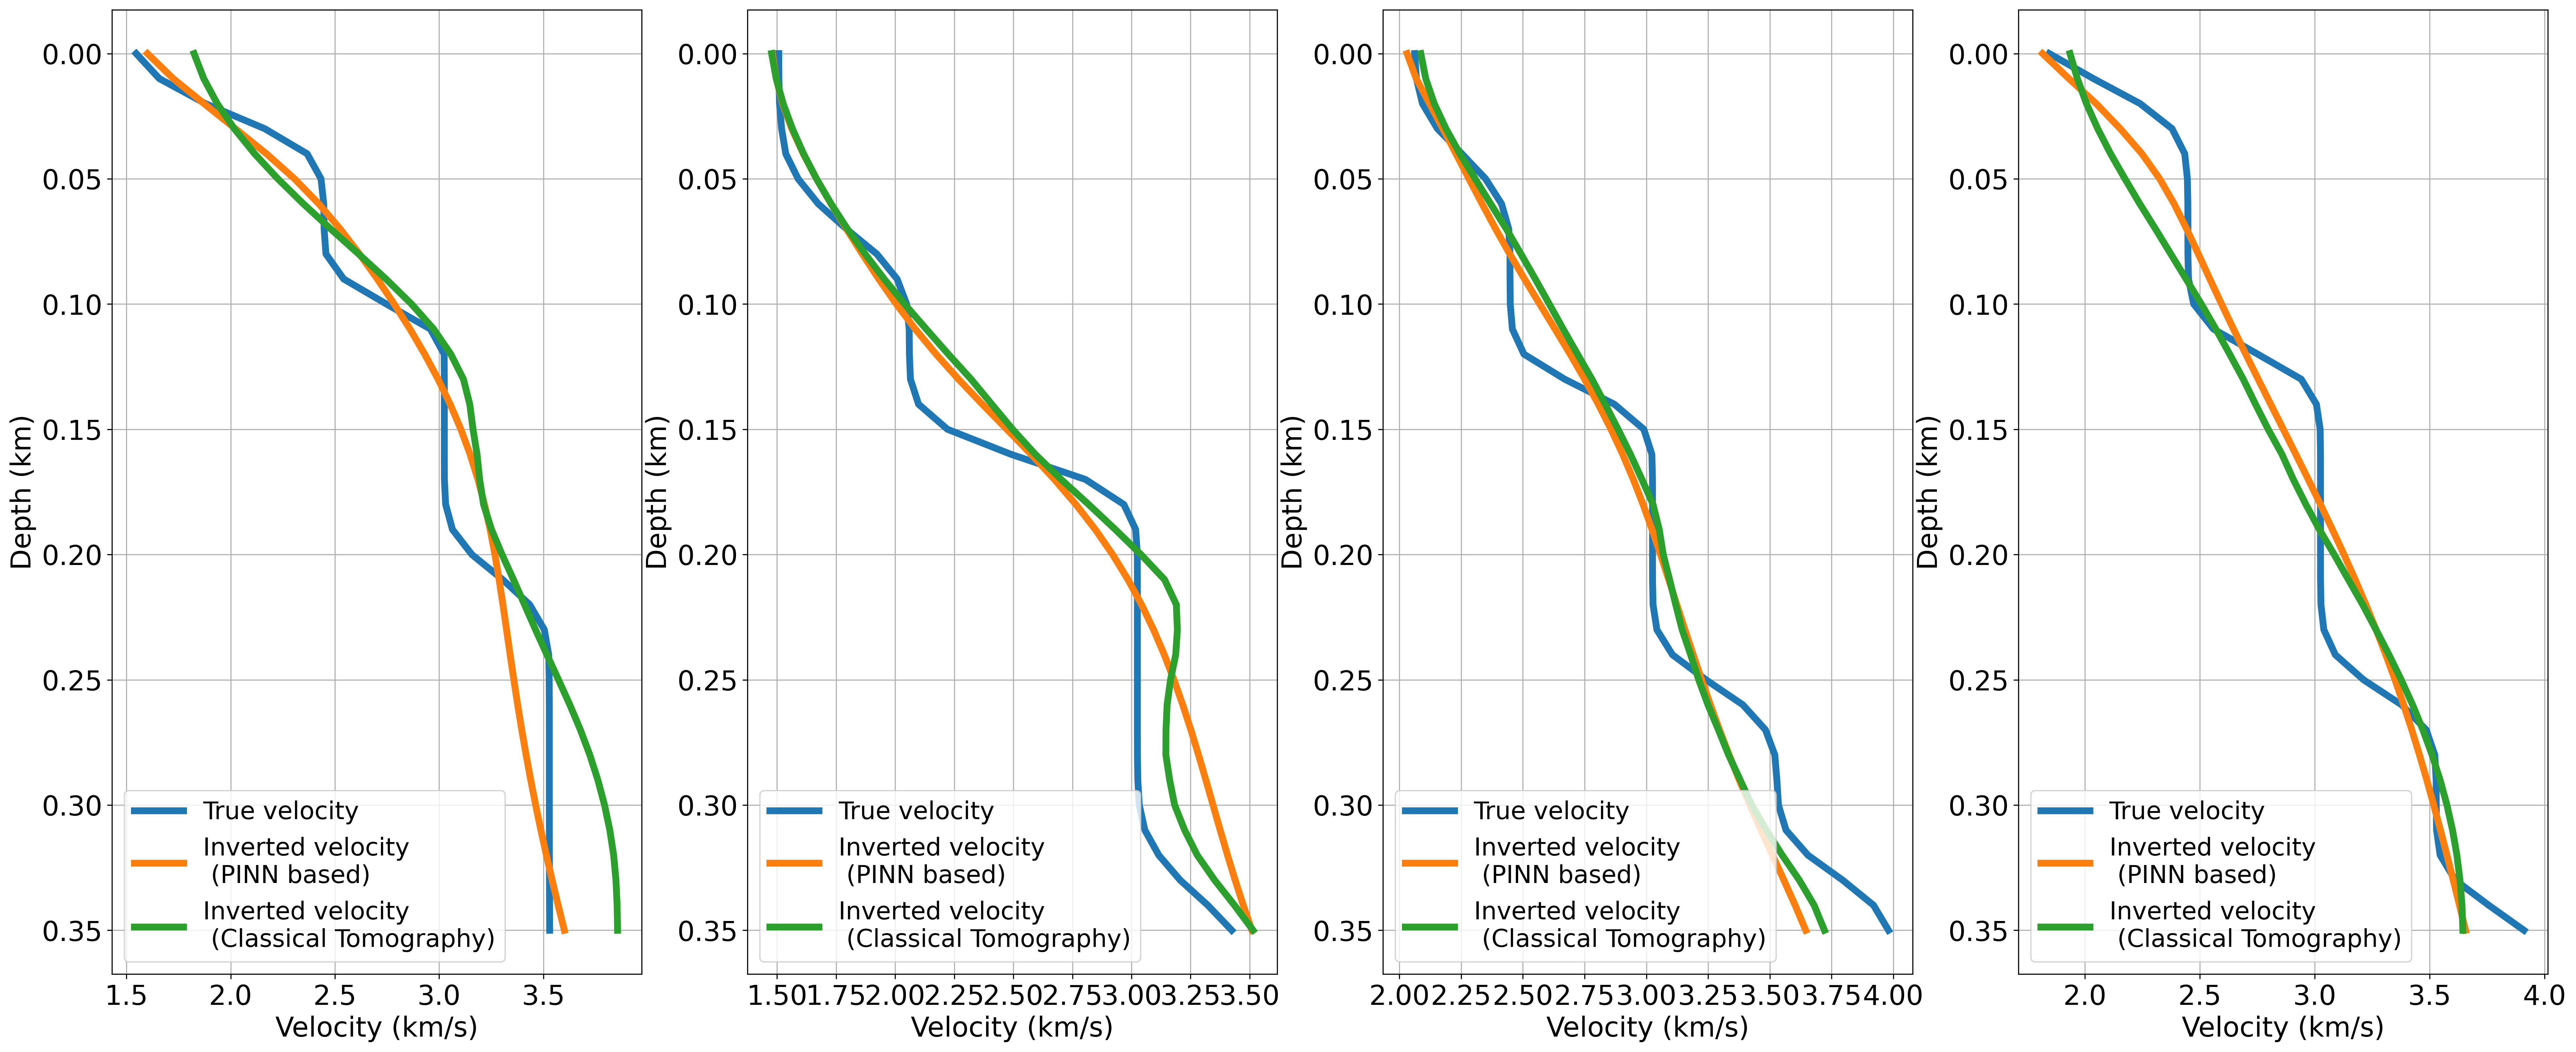
\includegraphics[width=0.9\textwidth]{figures/chap03_pinn_enabled/example_2_profiles} 
 \caption{Vertical velocity profiles at 0.4 km, 0.9 km, 1.3 km and 1.9 km from left to right respectively for the second example.}
 \label{fig:example_2_profiles}
\end{figure}

\begin{figure}
       \centering
       \begin{subfigure}[b]{1.\textwidth}
               \centering
               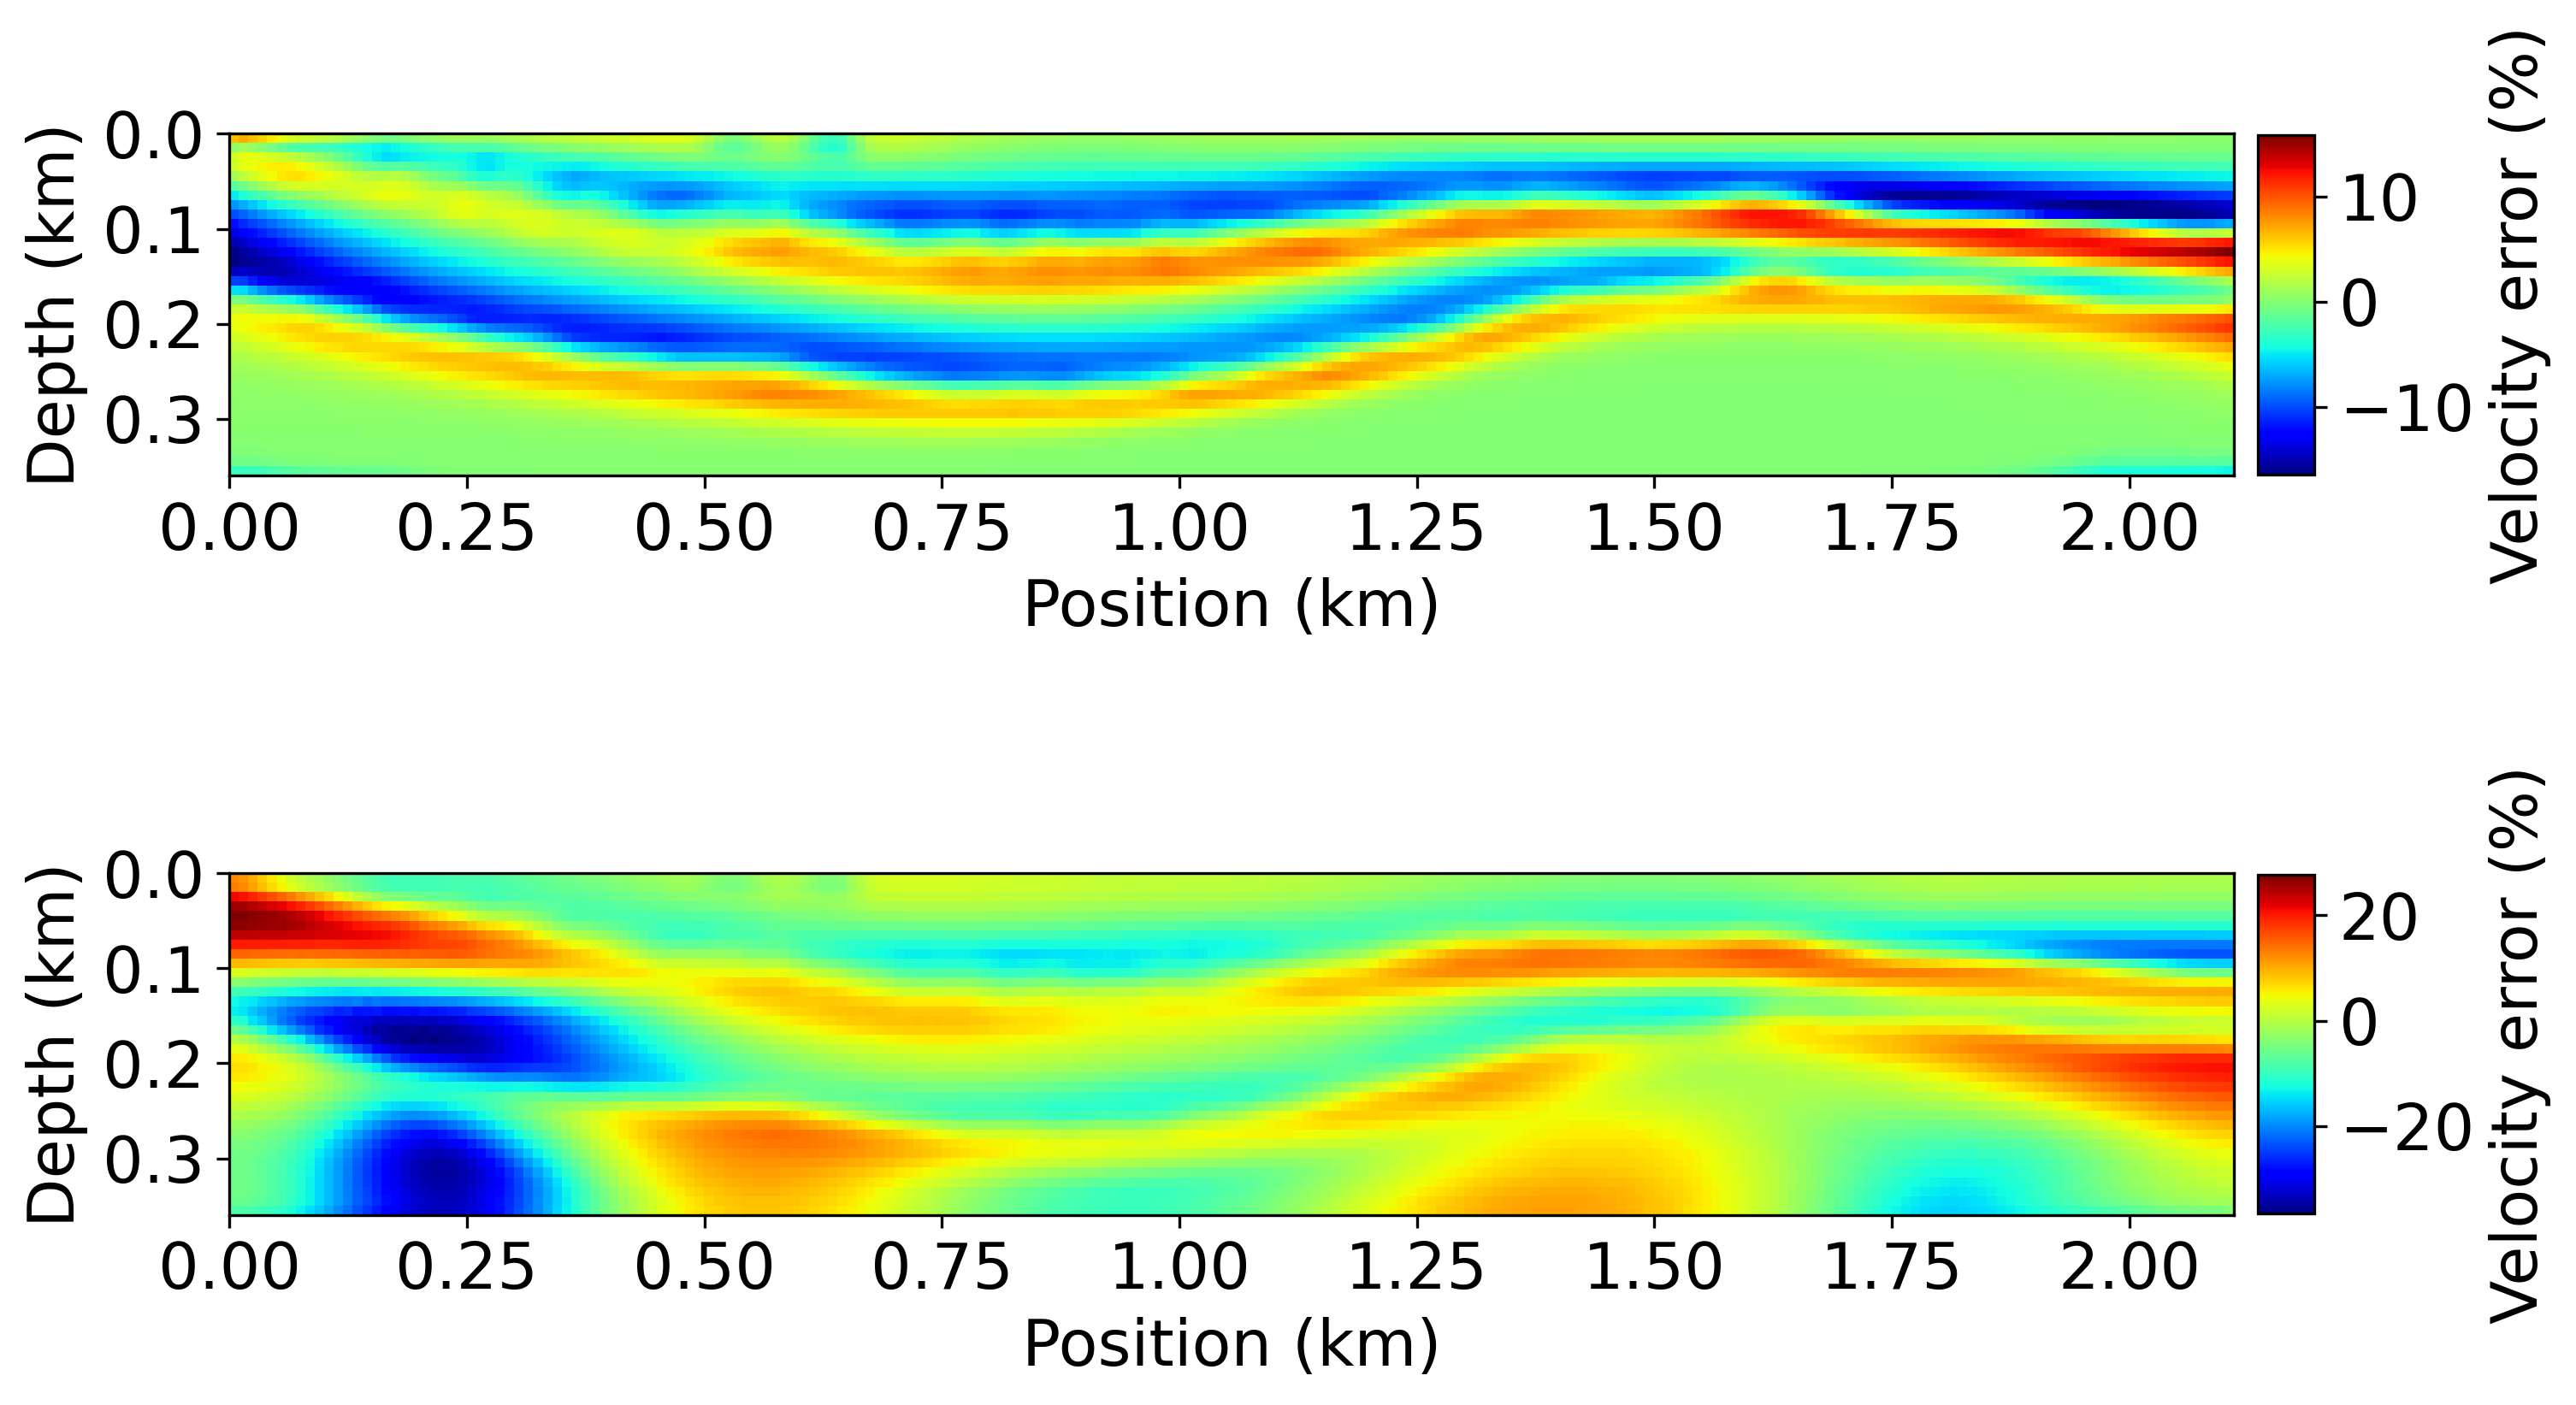
\includegraphics[width=\textwidth]{figures/chap03_pinn_enabled/example1_error} 
               \caption{}
               \label{fig:example1_error}
       \end{subfigure}
       %add desired spacing between images, e. g. ~, \quad, \qquad etc.
         %(or a blank line to force the subfigure onto a new line)
       \begin{subfigure}[b]{1.\textwidth}
               \centering
               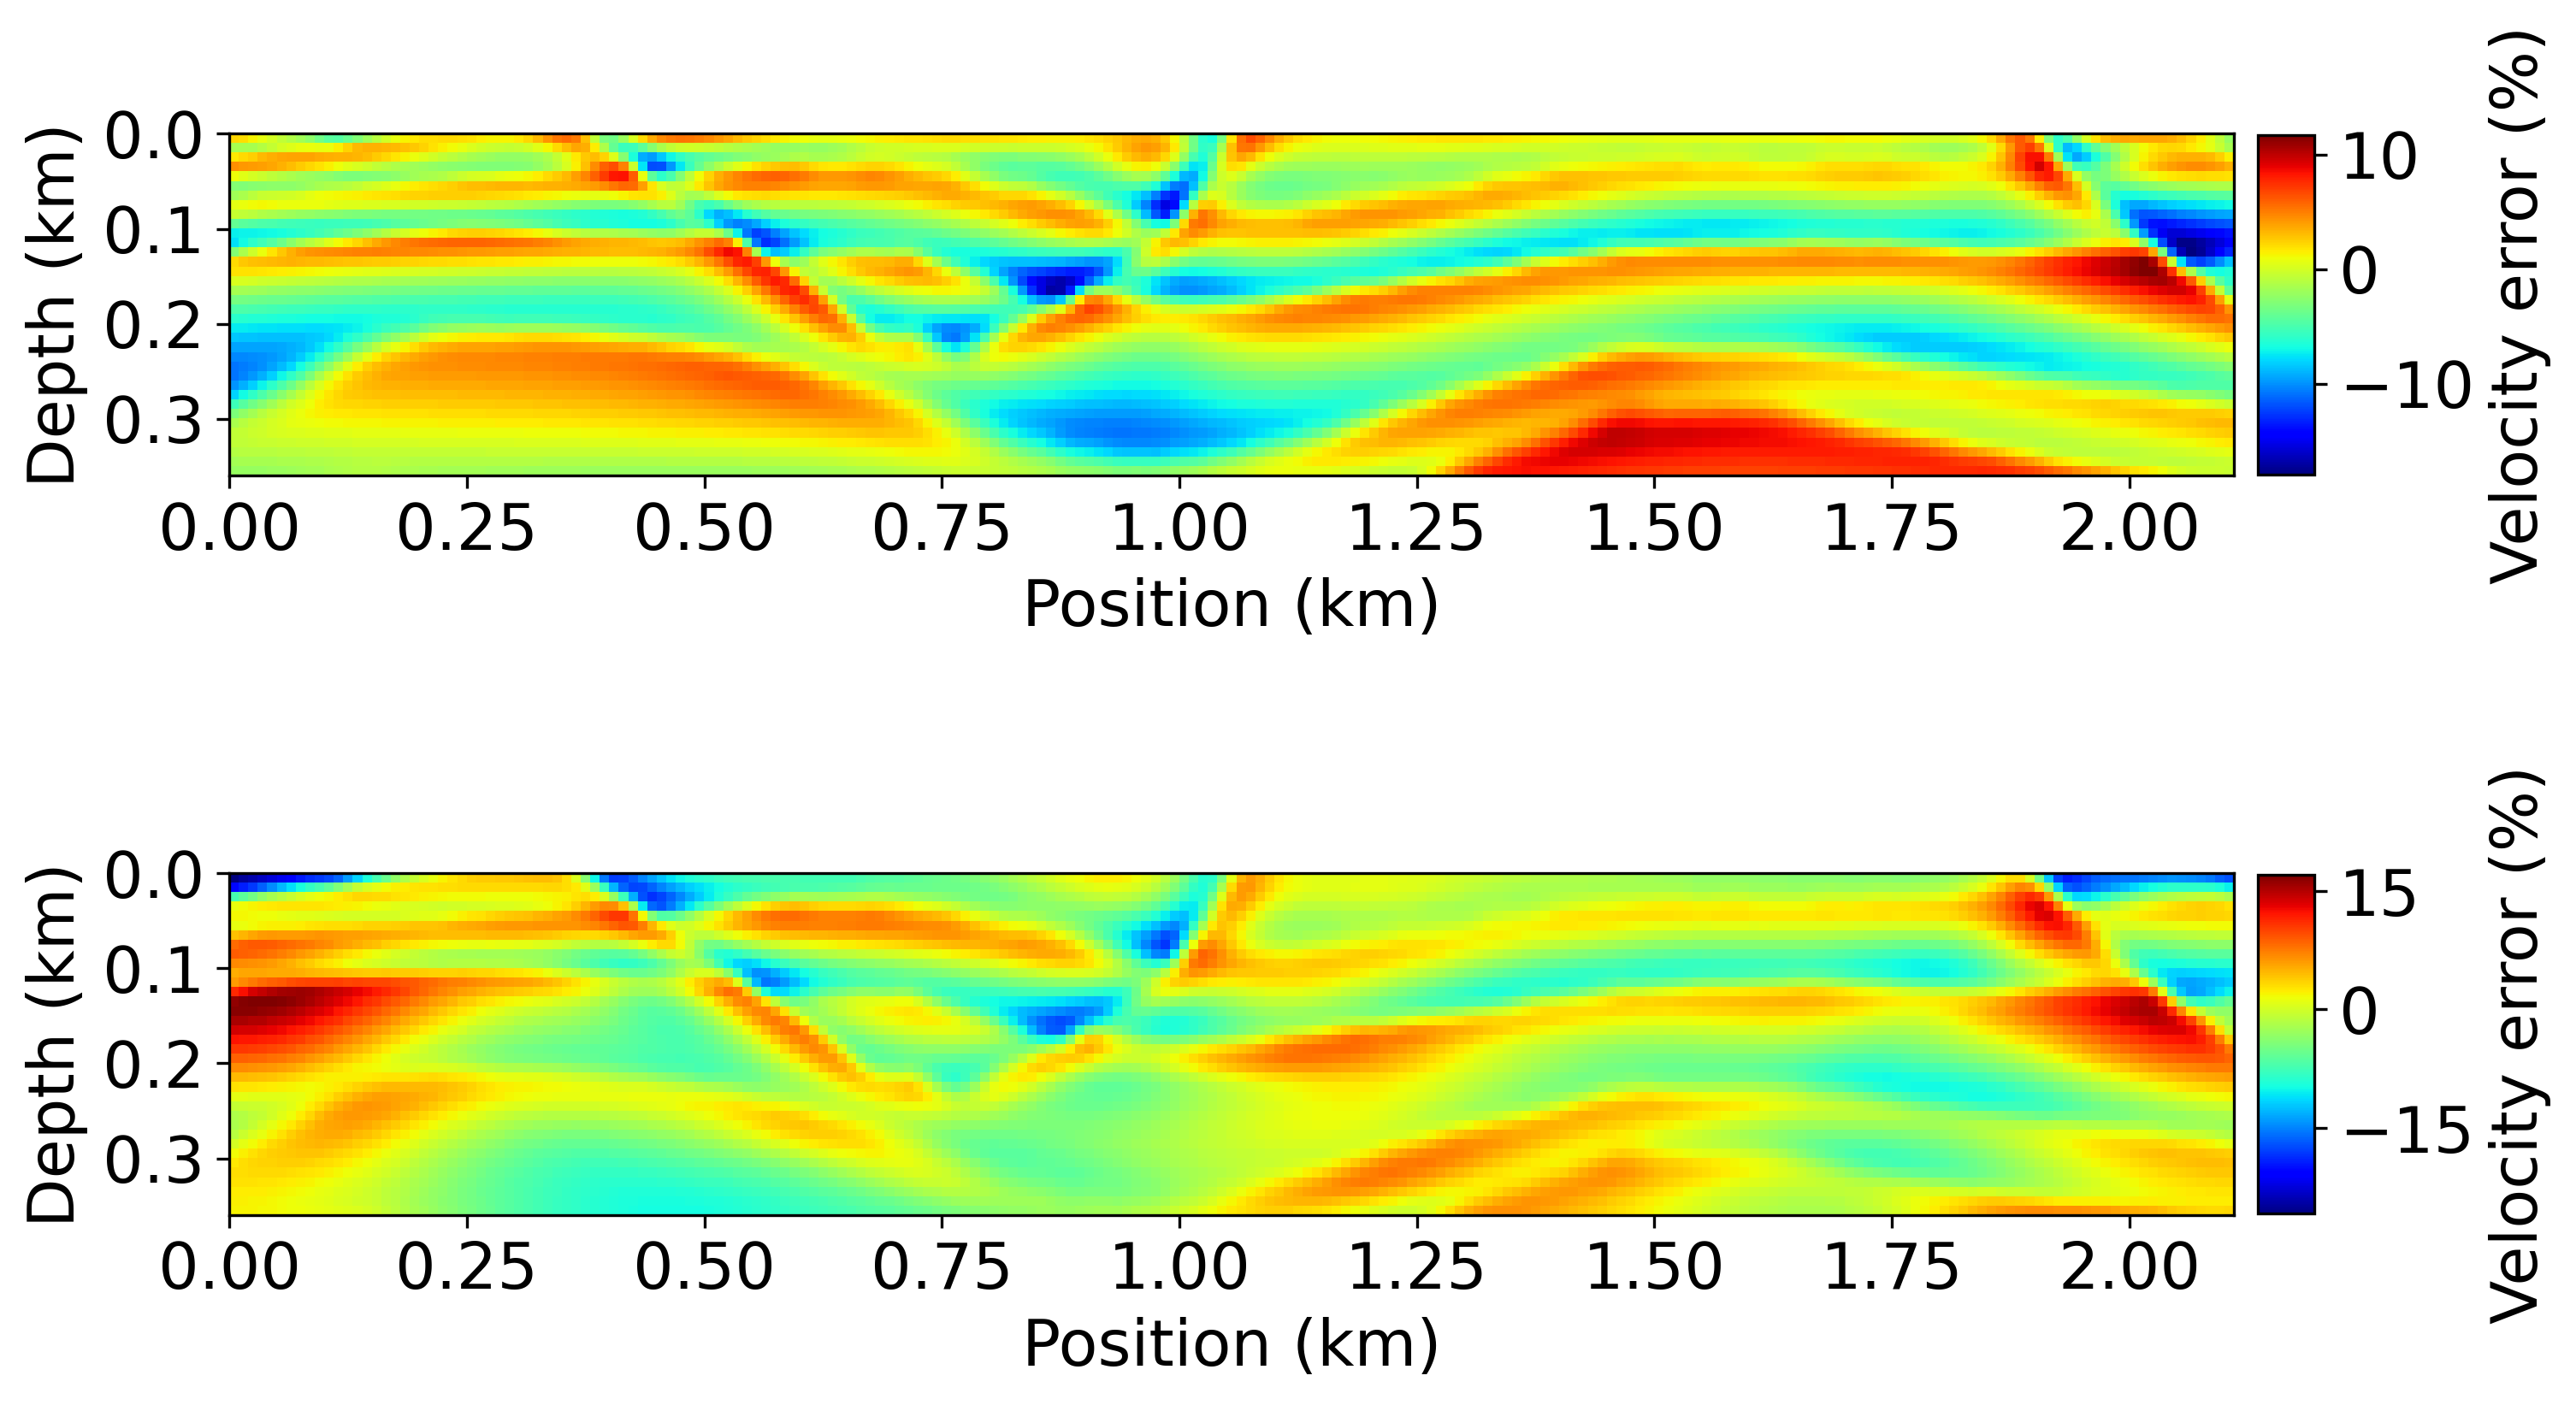
\includegraphics[width=\textwidth]{figures/chap03_pinn_enabled/example2_error}
               \caption{}
               \label{fig:example2_error}
       \end{subfigure}
       \caption{(a) Percentage error maps between the true model and the inversion results from the PINN approach (top) and the conventional approach (bottom) for the first example, and (b) for the second example, error map of PINN approach (top) and error map of conventional approach (bottom).}
       \label{fig:error}
\end{figure}